\section{Качество классификации}
Рассмотрим задачу бинарной классификации с обучающей выборкой $D = \{(x_i, y_i)\}_{i=1}^n$, где $x_i \in \mathbb{R}^d$ --- вектор признаков, $y_i \in \{0, 1\}$ --- бинарная переменная.
Мы хотим построить модель $f: \mathbb{R}^d \to \{0, 1\}$, которая принимает на вход вектор признаков и выдает предсказание класса.
Есть следующие способы измерять качество модели:

Accuracy

Precision

Recall

$F_{\beta}$ score

ROC AUC

Для каждого объекта из выборки мы имеем 4 варианта разивития событий:

TP --- True Positive, классификатор предсказал 1, верное значение тоже 1

FP --- False Positive, классификатор предсказал 1, верное значение 0

TN --- True Negative, классификатор предсказал 0, верное значение тоже 0

FN --- False Negative, классификатор предсказал 0, верное значение 1


Ясно, что мы хотим видеть как можно больше TP и TN и как можно меньше FP и FN.

Accuracy --- это доля правильных ответов классификатора.
$$
    \text{Accuracy} = \frac{TP + TN}{TP + FP + TN + FN} = \frac{1}{n} \sum_{i=1}^n \mathbb{I}(y_i = f(x_i))
$$

Достаточно банальная метрика, которая не учитывает дисбаланса классов, но в качестве базового варианта подходит отлично.

Precision --- это доля объектов, которые классификатор предсказал как 1, среди всех объектов, которые он предсказал как 1.
$$
    \text{Precision} = \frac{TP}{TP + FP}
$$

Recall --- это доля объектов, которые классификатор предсказал как 1, среди всех объектов, которые действительно равны 1.
$$
    \text{Recall} = \frac{TP}{TP + FN}
$$

Precision и Recall --- базовые метрики, но по отдельности их использовать нельзя, поэтому придумали $F_{\beta}$ score.

$F_{\beta}$ score --- это взвешенное среднее гармоническое precision и recall.
$$
    F_{\beta} = (1 + \beta^2) \frac{precision \cdot recall}{\beta^2 \cdot precision + recall}
$$

$TPR$ --- это доля объектов, которые классификатор предсказал как 1, среди всех объектов, которые действительно равны 1.
$$
    TPR = \frac{TP}{TP + FN}
$$

$FPR$ --- это доля объектов, которые классификатор предсказал как 1, среди всех объектов, которые действительно равны 0.
$$
    FPR = \frac{FP}{FP + TN}
$$

Обычно, когда мы решаем задачу бинарной классификации, то мы не предсказываем явный класс, а предсказываем какое-то значение, и чем больше это значение, тем больше вероятность того, что объект принадлежит к классу 1.
Следовательно, мы можем устанавливать пороговое значение, которое будет определять, к какому классу отнести объект.
При увеличении порога отсечения мы увеличиваем количество объектов, которые отнесены к классу 0, и уменьшаем количество объектов, которые отнесены к классу 1.
Заметим, что также при увеличении порога отсечения TPR и FPR будут уменьшаться.

ROC кривая --- это кривая, которая показывает зависимость TPR от FPR при изменении порога отсечения. То есть по оси $x$ откладывается $FPR$, а по оси $y$ --- $TPR$.

Строго говоря, ROC кривая --- это множество точек вида $(FPR(t), TPR(t))$, где $t$ --- пороговое значение вероятности.

ROC-AUC --- это площадь под ROC кривой.

\subsection*{Задача 1}

Мы хотим построить модель бинарной классификации, которая будет по некоторому описанию пациента предсказывать, болен ли он раком.
В случае, если наша модель скажет, что пациент болен раком, то мы отправим его на дополнительное обследование, что обойдется пациенту в некоторую неприятную, но не критичную сумму денег.
Если же наша модель скажет, что пациент здоров, то мы ничего не будем предпринимать.
Мы хотим выбрать метрику качества для нашей модели из следующего списка: Accuracy, Precision, Recall, $F_{\beta}$ score, что нам лучше всего подойдет?
Если мы хотим выбрать $F_{\beta}$ score, то какие значения $\beta$ нам лучше всего подойдут?

\subsection*{Решение}
Accuracy --- не лучший вариант, так как ошибка FP и FN в нашем случае не равнозначны.
Не отправить больного на дополнительное обследование значительно хуже, чем отправить здорового пациента на обследование.
Precision и Recall --- достаточно плохие метрики, ведь есть очень простая модель, которая даст 100\% Precision --- просто предсказывать, что все пациенты больны, аналогичная проблема и с Recall.
$F_{\beta}$ score --- отличный вариант, ведь с помощью $\beta$ мы можем выбирать, какое предпочтение мы отдаем Precision, а какое Recall.
В нашем случае, мы хотим, чтобы Precision был предпочтительнее Recall, поэтому $\beta$ должно быть меньше 1.
Если мы для себя решили, что смерть человека стоит как 10 дообследований, то стоит брать $\beta = \frac{1}{10}$.

\subsection*{Задача 2}
Предположим, что мы измеряем качество модели с помощью ROC-AUC. Допустим, что у нас есть две модели, чьи ROC кривые выглядят следующим образом:
\begin{figure}[h]
    \centering
    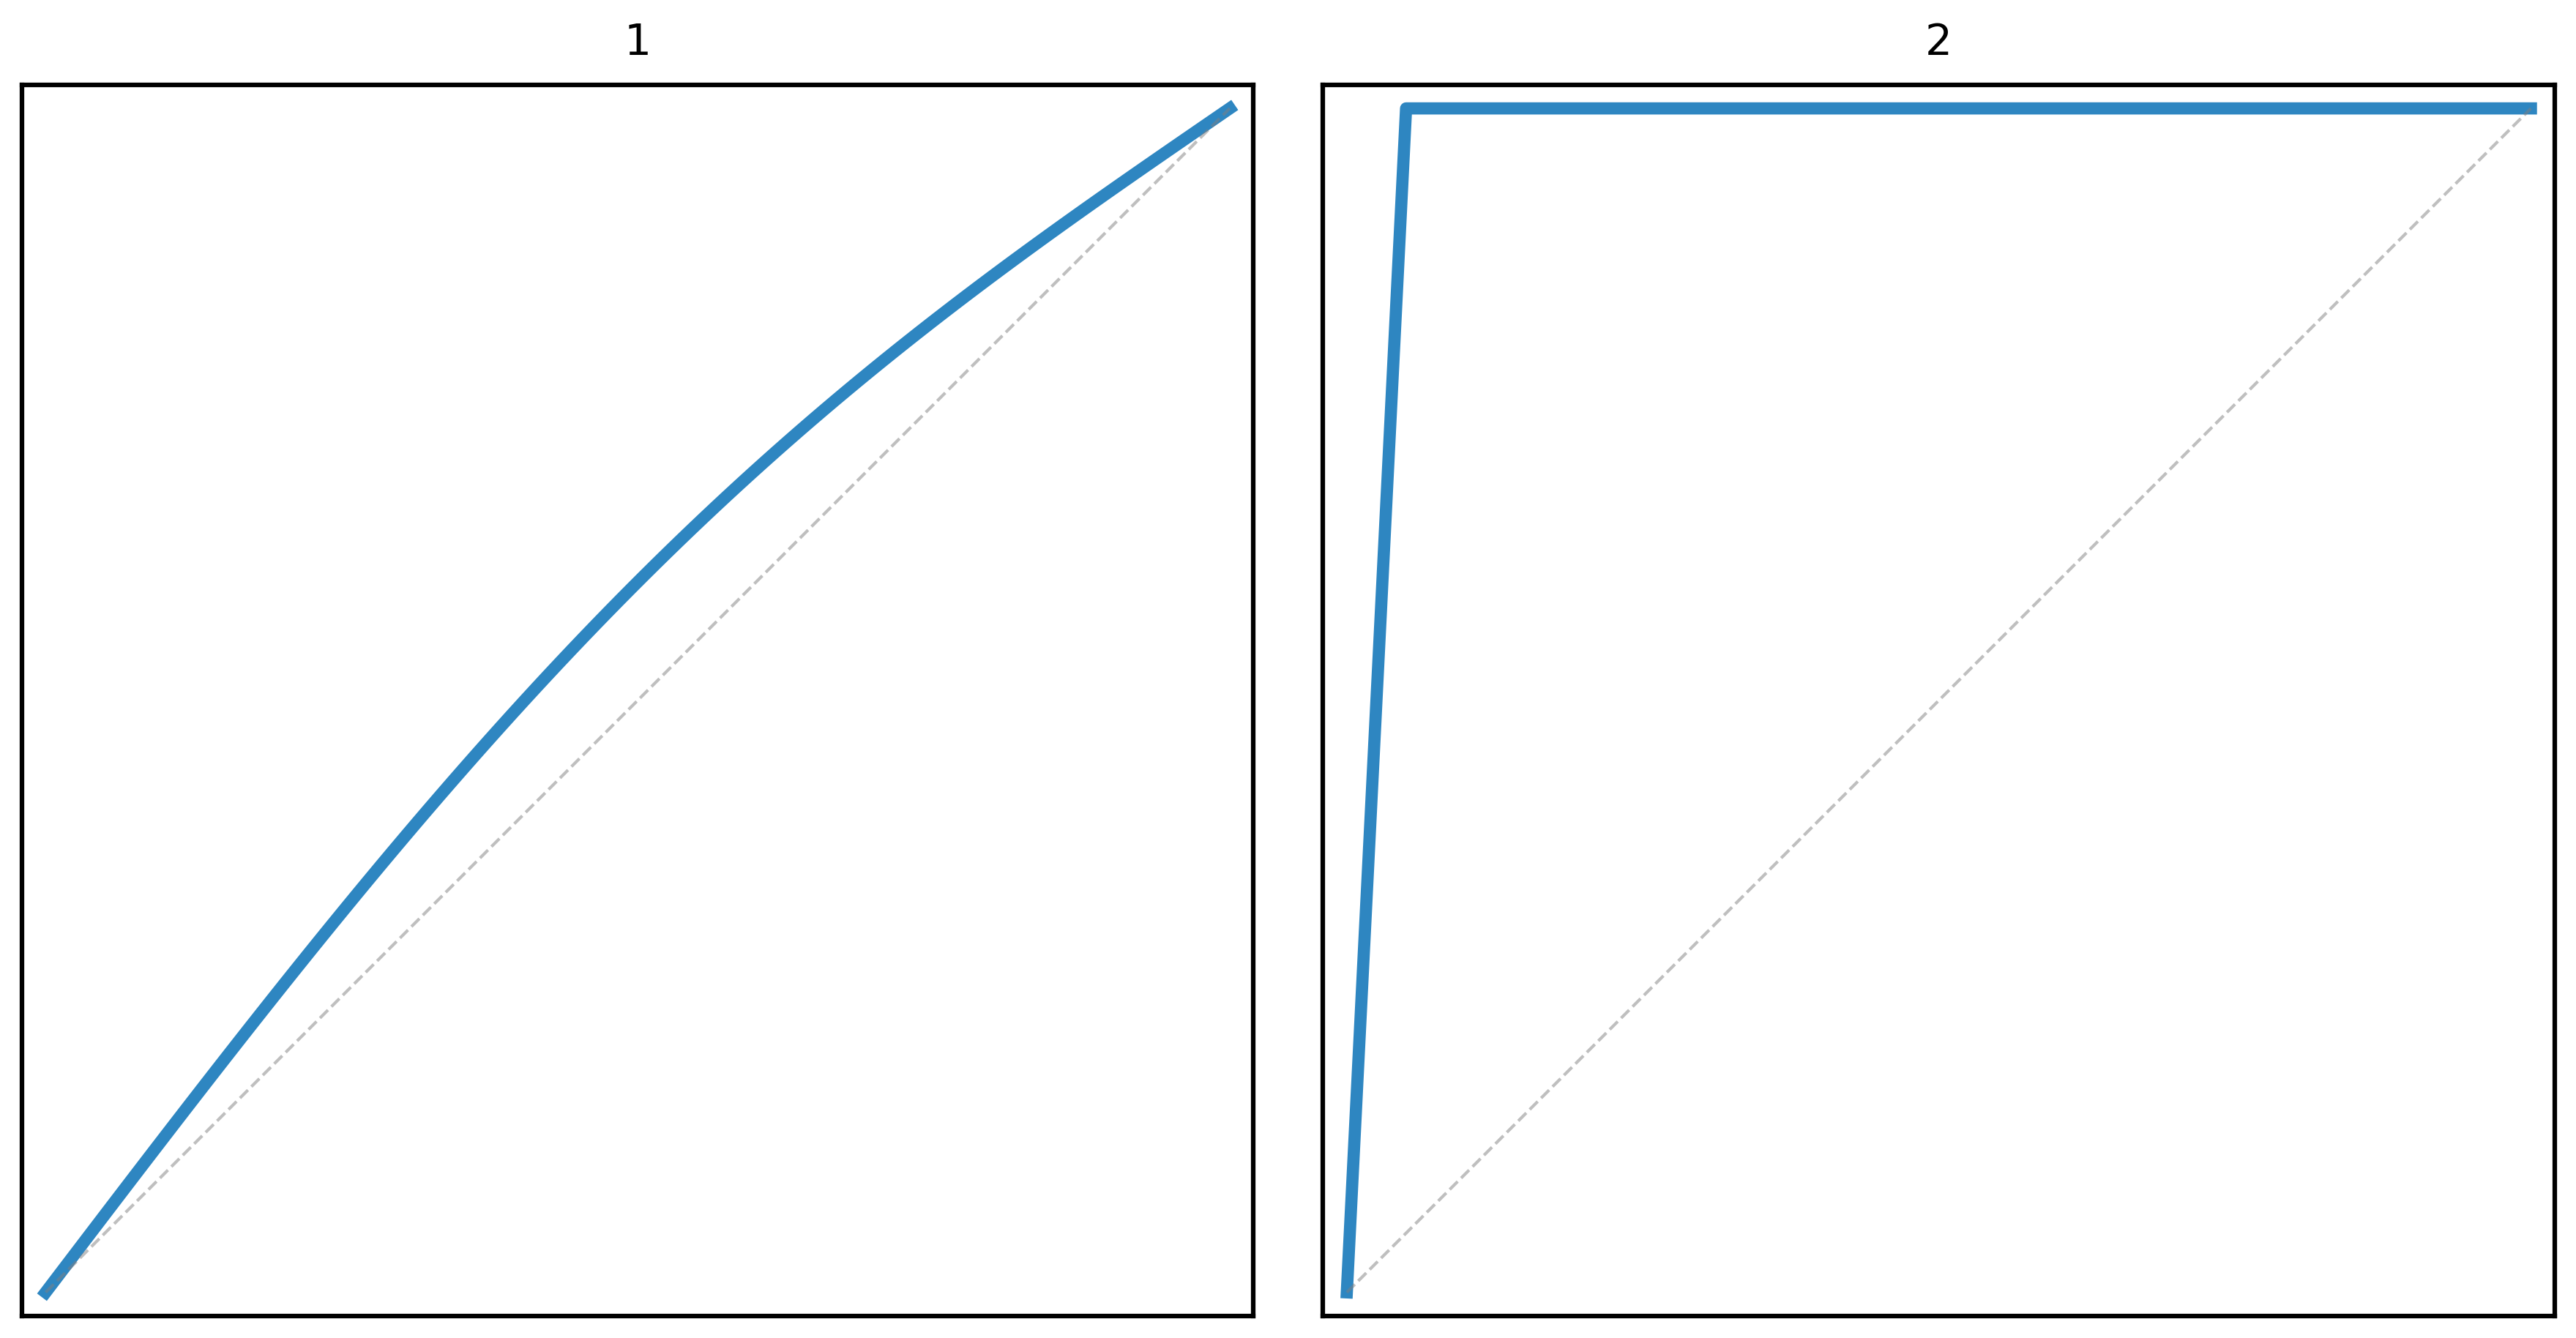
\includegraphics[width=0.8\textwidth]{chapters/feature_selection/roc_curves_comparison_1.png}
    \caption{Две ROC кривые}
\end{figure}
Как эти модели упорядочить по качеству?

\subsection*{Решение}
Первая модель самая худшая, ведь ее ROC кривая максимально близка к диагонали, значит она имеет миниимальную ROC-AUC.
Это плохо, но что по смыслу означает близкая к диагонали ROC кривая?

Это означает, что для любого порога отсечения $t$ имеем примерно $TPR(t) = FPR(t)$.
Что означает $TPR(t) = FPR(t)$? Это означает, что модель просто случайным образом с вероятностью $TPR(t)=FPR(t)$ предсказывает 1 класс.
Вторая модель лучшая, но почему?

А что означает график, который близок к уголку, как на рисунке 2?
Это означает, что мы можем взять такой порог отсечения $t$, что почти выполнено $TPR(t) = 1$ и $FPR(t) = 0$.
А это идеальная модель, которая никогда не ошибается.

Заметим, что чем больше площадь под ROC кривой, тем ближе эта кривая к уголку, а значит тем лучше модель.

\subsection*{Задача 3}
Продолжим измерять качество моделей с помощью ROC-AUC. Допустим, что у нас есть две модели, чьи ROC кривые выглядят следующим образом:
\begin{figure}[h]
    \centering
    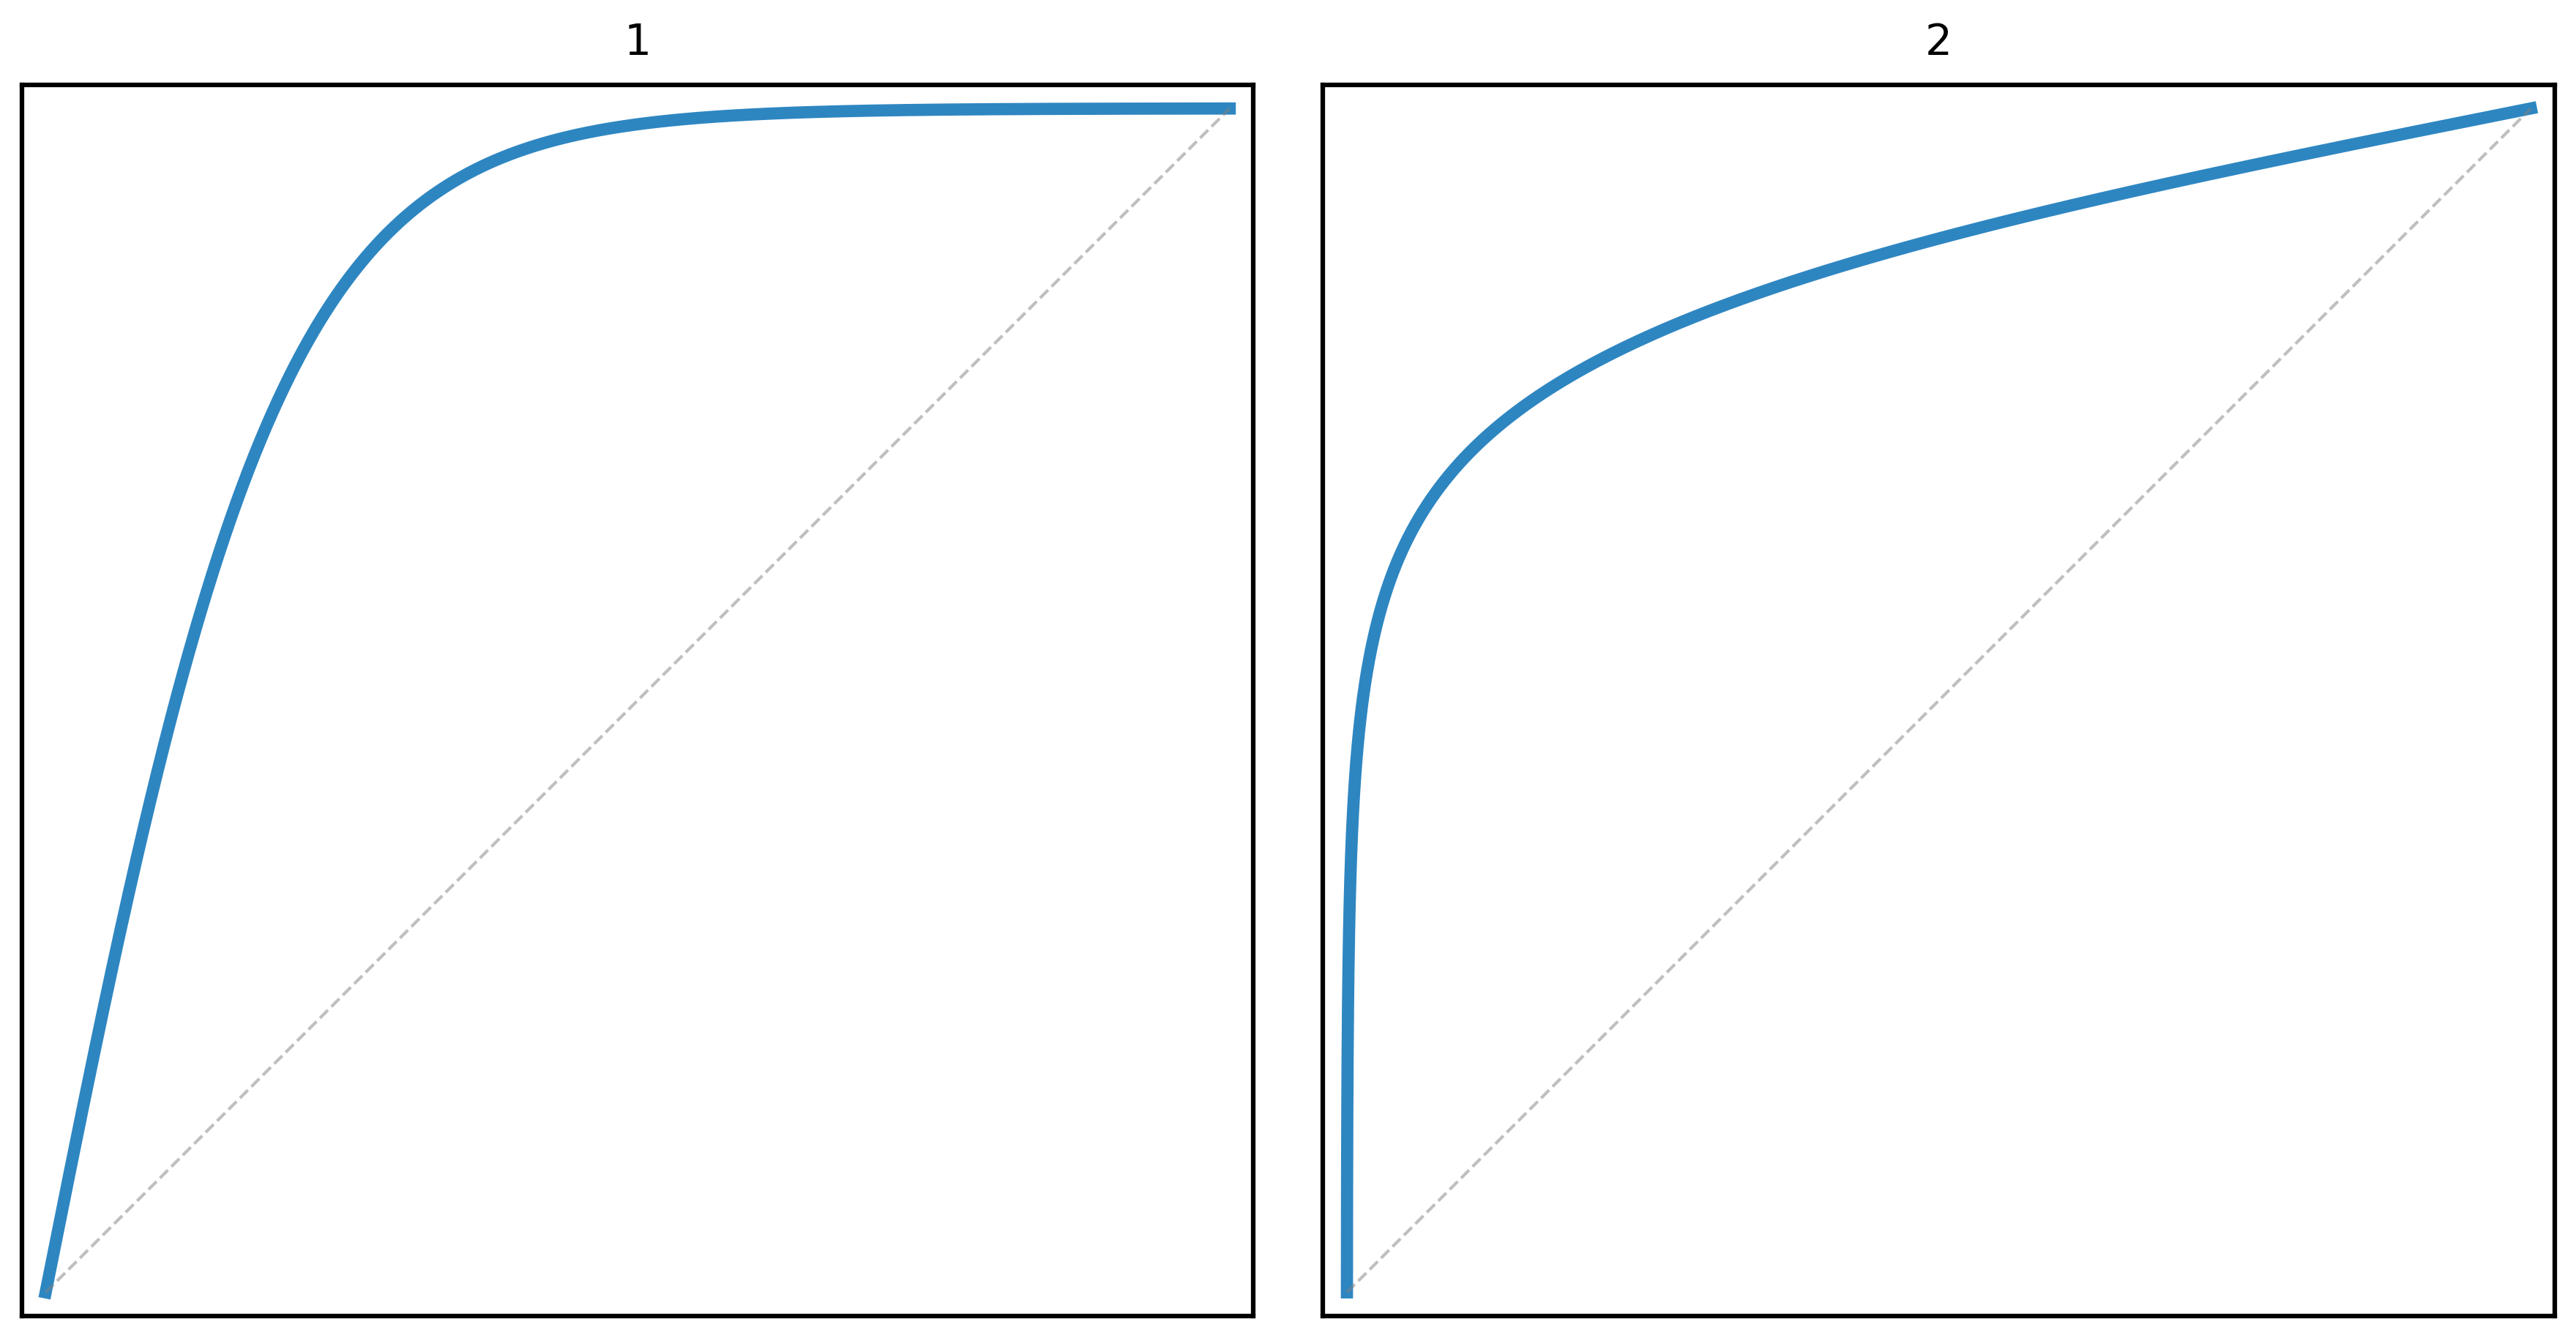
\includegraphics[width=0.8\textwidth]{chapters/feature_selection/roc_curves_comparison_2.png}
    \caption{Две ROC кривые}
\end{figure}
Как эти модели упорядочить по качеству? А как выбрать порог отсечения? В чем преимущество ROC перед $F_{\beta}$ score?

\subsection*{Решение}
В данном случае, обе ROC кривые имеют одинаковую площадь под графиком, а значит одинаковую ROC-AUC, поэтому просто посмотреть на метрику ROC-AUC нельзя.
На самом деле, однозначного ответа нет, всё зависит от конкретной задачи.

Первая кривая быстро достигает высокого значения TPR, при не самом высоком значении FPR.

Это означает, что выбрав порог отсечения $t$, при котором $TPR(t)$ будет близок к 1, а $FPR(t)$ будет близок к 0.5, мы получим модель,
которая угадывает почти всех, кто попадает в 1 класс, но при этом не сильно много ошибается на классе 0.
Такая модель отлично подойдет в первой задаче, где мы хотим отгадать почти всех больных, но при этом не сильно много отправлять на дополнительное обследование здоровых людей.

На втором графике ситуация обратная, мы можем выбрать порог отсечения $t$, при котором $TPR(t)$ будет близок к 0.5, а $FPR(t)$ будет близок к 1.
Такая модель будет полезна в случае, когда мы хотим минимизировать количество ошибок на классе 0, но при этом не сильно много ошибаться на классе 1.
В контексте первой задачи, это означает, что мы не хотим тратить лишние деньги на дополнительное обследование здоровых людей даже ценой смерти больных, которых мы не отправляем на дополнительное обследование.

Исходя из этих примеров, становится понятно, как стоит выбирать порог отсечения. По сути его выбор означает, насколько мы готовы пожертвовать ошибками на предсказаниях одного класса, чтобы минимизировать ошибки на предсказаниях другого класса.
Это такой аналог $\beta$ в $F_{\beta}$ score, только $\beta$ мы выбирали до измерения метрики, а в случае ROC кривой мы выбираем порог отсечения глядя на график и имея какую-то дополнительную информацию о том, как работает модель при разных порогах.
Это может быть очень полезно, ведь далеко не всегда мы готовы определиться с балансом ошибок на классах перед тем, как начать решать задачу.


\section{Методы отбора признаков: полный перебор, алгоритм Add}

Работа с признаками включает два основных подхода:
\begin{enumerate}
    \item Генерация новых признаков;
    \item Отбор существующих признаков.
\end{enumerate}

\subsection{Генерация новых признаков}
Генерация новых признаков подразумевает создание таких признаков, которые представляют собой преобразованные версии исходных данных или полностью новые параметры, полученные из имеющихся данных. Примеры методов генерации признаков включают:

\begin{itemize}
    \item Построение статистик на основе существующих признаков (например, среднее, стандартное отклонение, медиана и т.д.);
    \item Использование методов понижения размерности, таких как анализ главных компонент (PCA);
    \item Применение нейросетей, где скрытые слои (за исключением последнего) могут рассматриваться как новое, более информативное признаковое пространство.
\end{itemize}

В этой главе мы сосредоточимся на отборе существующих признаков, рассмотрев два наиболее популярных метода: полный перебор и жадный алгоритм Add.

\subsection{Полный перебор}

Метод полного перебора представляет собой один из самых простых и технически точных подходов к отбору признаков. Суть метода заключается в оценке качества модели на всех возможных комбинациях признаков и выборе той комбинации, которая обеспечивает наилучшую метрику. Таким образом, полный перебор \textbf{гарантирует нахождение оптимального набора признаков}, так как проверяет все возможные варианты.

Основное преимущество полного перебора заключается в его точности: при достаточных вычислительных ресурсах метод всегда найдёт лучшее решение. Тем не менее, с увеличением числа признаков $n$, количество возможных подмножеств растёт экспоненциально ($2^n$). Это делает полный перебор крайне ресурсоёмким для наборов данных с большим $n$. Например, уже при $n=20$ потребуется рассчитать $2^{20} = 1,048,576$ комбинаций.

Метод полного перебора чаще применяется:
\begin{itemize}
    \item Для небольших наборов признаков, где перебор возможен за приемлемое время;
    \item В задачах, где цена ошибки высока (например, в медицинских исследованиях);
    \item Когда требуется хорошая интерпретируемость и точность подмножеств признаков.
\end{itemize}

На больших данных иногда применяются модификации полного перебора, такие как частичный перебор, где анализируется только часть комбинаций (например, сначала отбираются наиболее значимые признаки с помощью другого метода, а затем производится перебор подмножеств только из этих признаков).

\subsection{Жадный алгоритм Add}

Алгоритм Add (жадный подход) используется гораздо чаще, чем полный перебор, благодаря лучшей производительности на больших данных и более простой интерпретации. Суть метода заключается в пошаговом добавлении признаков в модель. На каждом шаге из оставшихся признаков выбирается тот, который обеспечивает наибольшее улучшение метрики модели. Таким образом, итоговый набор строится итеративно, начиная с пустого множества и поочередно добавляя наиболее значимые признаки.

Жадный алгоритм не гарантирует нахождения глобального оптимума, так как выбирает локально лучшие решения на каждом из шагов. Однако его высокая скорость и способность работать с большими наборами признаков делают его востребованным для многих задач.

Очевидно, что из общего числа признаков $n$ должен остаться некоторый $k$-подмножество наиболее значимых признаков. Критерии остановки алгоритма Add могут быть следующими:

\begin{itemize}
    \item \textbf{Фиксированное количество признаков $k$}:  
    Алгоритм останавливается, как только выбрано заданное количество признаков $k$.  
    \textit{Плюсы:} простота реализации и возможность заранее контролировать размерность данных.  
    \textit{Минусы:} фиксированное значение $k$ может оказаться избыточным в одной задаче или недостаточным в другой. Чтобы минимизировать неопределённость, значения параметра $k$ можно подбирать по сетке с помощью кросс-валидации.
    
    \item \textbf{Остановка при отсутствии улучшения метрики}:  
    На каждом шаге проверяется, насколько новая комбинация признаков улучшает метрику модели (например, \(R^2\), \(MAPE\), RMSE). Если добавление нового признака не приводит к значимому улучшению (или ухудшает метрику), алгоритм прекращает выполнение.  
    \textit{Плюсы:} гибкость метода, так как он адаптируется к конкретной задаче.  
    \textit{Минусы:} возможно преждевременное завершение, если данные содержат шум.
\end{itemize}

Метод Add применяется, когда требуется построить интерпретируемую модель с допустимым уровнем качества за ограниченное время. Например, алгоритм широко используется в финансах для выделения ключевых факторов прогнозирования прибыли или моделирования рисков, а также в обработке медицинских данных. 

\textbf{Преимущества метода Add:}
\begin{itemize}
    \item Высокая скорость работы и масштабируемость для большого числа признаков;
    \item Возможность построить достаточно простую и интерпретируемую модель.
\end{itemize}

\textbf{Недостатки метода Add:}
\begin{itemize}
    \item Чувствительность к входным данным: выбросы и избыточные признаки могут искажать отбор на ранних этапах;
    \item Отсутствие глобальной оптимальности: алгоритм может игнорировать комбинации признаков, т.к. учитывает только влияние признаков по отдельности.
\end{itemize}

\subsection{Задачи}

\subsubsection{Задача 1.}

Есть набор данных с N = 10000 признаков, и задача состоит в отборе важных признаков. Отбор происходит с помощью метода Add, но на каждом шаге анализ всех оставшихся признаков (выбор из 10000, затем из 9999 и т.д.) занимает слишком много времени.

Как можно было бы улучшить этот метод?

\subsubsection{Ответ 1.}

Можно разделить все признаки случайным образом на блоки (например, по 100 признаков). В таком случае хорошей идеей будет выбрать лучший признак из каждого блока на предварительном этапе (т.е. жадный Add выполняется на подмножествах сначала локально в блоках), а затем продолжить работу с меньшим числом представителей от каждых блоков. Если блоки и так большого размера, то можно воспользоваться этой идеей рекурсивно для каждого подблока.

\subsubsection{Задача 2.}

Рассмотрим использование жадного алгоритма Add для выбора признаков из набора данных с 5 признаками ({A, B, C, D, E}) в задаче классификации.

График перезаписи последовательного роста метрики $R^2$ при добавлении выбранных признаков показан ниже:

\begin{table}[h!]
\centering
\begin{tabular}{|c|c|c|}
\hline
\textbf{Итерация} & \textbf{Добавленный признак} & \boldmath${R^2}$ \\ \hline
1                 & $A$                       & 0.45             \\ \hline
2                 & $B$                       & 0.53             \\ \hline
3                 & $C$                       & 0.58             \\ \hline
\end{tabular}
\end{table}

Между тем, известна модель из полного перебора, где признаковая комбинация $({A, D, E})$ даёт $R^2 = 0.67$.

Почему метод Add мог не найти эту комбинацию? Как можно было бы исправить эту ситуацию и повысить вероятность нахождения глобального оптимума?

\subsubsection{Ответ 2.}

Жадный алгоритм Add выбирает признак на каждом шаге, который локально улучшает метрику максимально. Однако комбинация $({A, D, E})$ могла быть значимой только в сочетании (то есть признаки дают прирост метрики только в комбинации), а по отдельности эти фичи дают не такой хороший прирост к метрике, как $B$ и $C$. Add не проверяет взаимодействие признаков, поэтому выбор локально наилучших признаков $({A, B, C})$ мог игнорировать комбинацию, которая глобально лучше.

\textbf{Как с этим можно бороться?}
\begin{itemize}
    \item Проверять метрику при добавлении не одного признака, а пары/тройки/произвольного числа $m$ признаков.
    \item Использовать модификацию жадного алгоритма с дополнительными "прыжками", то есть, например, после 3 итераций Add можно сделать перезапуск среди лучших комбинаций 2 признаков.
\end{itemize}

\subsubsection{Вопрос 3.}

Есть набор данных с 20 признаками. Известно, что 10 из них абсолютно не связана с целевой переменной, т.е. являются шумовыми. Однако не известно, какие именно из них являются шумовыми. Для отбора признаков был применен жадный алгоритм Add.

Предположим, что на первых итерациях жадный алгоритм случайно выбрал несколько шумовых признаков, так как они хорошо улучшили метрику на обучающей выборке.

Как это повлияет на работу алгоритма Add в следующих итерациях? Какие подходы вы бы предложили, чтобы минимизировать вероятность включения шумовых признаков на ранних этапах?

\subsubsection{Ответ 3.}\

\textbf{1. Как это повлияет на дальнейшую работу алгоритма?}

Жадный алгоритм фиксирует признаки и рассматривает следующие шаги на основе текущего набора. Если шумовые признаки остаются в модели, они могут "вытеснять" более значимые признаки в дальнейших итерациях.
Итоговый результат может быть хуже, так как модель становится менее интерпретируемой и более склонной к переобучению на шум.

\textbf{2. Как можно минимизировать влияние шума на обучение?}

Для этого стоит перед алгоритмом применить другие фильтрационные методы для удаления явно нерелевантных признаков, например, убрать признаки, плохо коррелирующие с целевой переменной.

Также для этого можно попробовать применить кросс-валидацию при оценке каждого нового признака, чтобы убедиться, что он действительно улучшает модель (а не только улучшает метрику на обучающей выборке).

\section{Методы преобразования категориальных признаков}

Категориальные признаки (или категориальные переменные) — это тип данных, который представляет собой категории или группы. В отличие от количественных признаков, которые принимают числовые значения, категориальные признаки описывают качественные характеристики.

\begin{itemize}
	\item Номинальные признаки -- эти признаки представляют собой категории, которые не имеют никакого порядка (город, где проживает человек; цвет машины).
	\item Порядковые признаки -- эти признаки также представляют категории, но в отличие от номинальных, они имеют естественный порядок (уровень образования; степень удовлетворенности).
\end{itemize}

Такие признаки невозможно напрямую использовать в моделях машинного обучения, поскольку они работают с числами. Для решения этой проблемы есть различные методы.

\subsection*{One-hot (dummy) encoding}

One-hot encoding — это метод кодирования категориальных переменных, который преобразует каждую категорию в бинарный вектор, где только один элемент равен 1 (представляет категорию), а все остальные элементы равны 0.

Преимущества:
\begin{itemize}
	\item Он легко реализуется, а данные легко интерпретируются.
	\item Хорошо совместим почти со всеми алгоритмами.
	\item Подходит для изначально неупорядоченных данных.
\end{itemize}

Недостатки:
\begin{itemize}
	\item В случае большого количества категорий сильно увеличивает размерность, может привести к переобучению.
	\item Полученные признаки сильно разреженны, неэффективно по памяти и скорости вычислений.
	\item Не подходит для упорядоченных или взаимосвязанных данных.
\end{itemize}

\subsection*{Effect (treatment, deviation) encoding}

Effect encoding  — это метод кодирования категориальных переменных, который представляет каждую категорию в виде разности между средним значением целевой переменной и средними значениями для каждой категории. Этот метод позволяет учитывать информацию о влиянии каждой категории на целевую переменную.

Преимущества:
\begin{itemize}
	\item Сохраняет информацию о влиянии категории на целевую переменную.
	\item Не увеличивает размерность пространства признаков.
	\item Создает порядок между категориями, основываясь на значении целевой переменной.
\end{itemize}

Недостатки:
\begin{itemize}
	\item Не так прост для интерпретации, как one-hot encoding.
	\item Может создать многократную коллинеарность между несколькими категориальными признаками.
\end{itemize}

\subsection*{Label (ordinal) encoding}

Label encoding — это метод кодирования категориальных переменных, при котором каждой категории присваивается уникальное целочисленное значение.

Преимущества:
\begin{itemize}
	\item Прост в реализации.
	\item Не увеличивает размерность пространства признаков.
	\item Сохраняет информацию порядковых признаков.
	\item Хорошо совместим с алгоритмами, не зависящими от расстояния между значениями (деревья решений).
\end{itemize}

Недостатки:
\begin{itemize}
	\item Создает ложный порядок в номинальных признаках.
	\item Плохо совместим с линейными моделями.
	\item Создает ложные расстояния между категориями.
\end{itemize}

\subsection*{Count encoding}

Count encoding — это метод кодирования категориальных переменных, при котором каждой категории присваивается количество её появлений в наборе данных. 
	
Преимущества:
\begin{itemize}
	\item Прост в реализации.
	\item Сохраняет информацию о частоте.
	\item Не увеличивает размерность пространства признаков.
\end{itemize}

Недостатки:
\begin{itemize}
	\item Не сохраняет информацию порядковых признаков.
	\item Может создать коллинеарность для разных категорий с близкими частотами.
	\item Создает ложные расстояния между категориями.
\end{itemize}

\subsection*{Задача 1}

В случае использования one-hot encoding для категориального признака с $N$ уникальными значениями, мы получим $N$ новых признаков. Однако любой признак выражается через остальные, поскольку единица всегда стоит только в одном из них. То есть мы получили мультиколлинеарность, которая может ухудшить качества модели! Каким образом можно решить эту проблему?

\subsection*{Решение}

Самым простым решением будет просто удалить любой из полученных признаков. Мы избавимся от мультиколлинеарности и сохраним всю информацию о выборке.

\subsection*{Задача 2}

Проведите преобразование категориальных признаков по методу effective encoding:
\begin{table}[ht]
	\footnotesize
	\begin{tabular}{lllll}
		\hline
		Пробег, тыс. км & Цвет    & Год выпуска & Тип кузова & Стоимость, у.е. \\ \hline
		100             & Красный & 2015        & Хэтчбэк    & 10           \\
		10              & Зеленый & 2019        & Cедан      & 17           \\
		17              & Cиний   & 2022        & Cедан      & 18           \\
		150             & Красный & 2019        & Универсал  & 15           \\
		30              & Красный & 2023        & Хэтчбэк    & 20           \\
		174             & Cиний   & 2017        & Хэтчбэк    & 12           \\
		89              & Зеленый & 2017        & Хэтчбэк    & 14           \\ \hline
	\end{tabular}
\end{table}

\subsection*{Решение}

Для каждого цвета вычислим средние значение стоимости:
\begin{itemize}
	\item Красный: $r = \frac{10+15+20}{3}=15$.
	\item Зеленый: $g = \frac{17+14}{2}=15.5$.
	\item Синий: $b = \frac{18+9}{2}=13.5$.
\end{itemize}

Тогда среднее для всех признаков:
$$ avg = \frac{15 + 15.5 + 13.5}{3} = 14.66. $$

Значение нового признака, например, для красного цвета:
$$ r - avg = 0.33. $$

\begin{table}[ht]
	\footnotesize
	\begin{tabular}{lllllll}
		\hline
		Пробег, тыс. км & Цвет    & Год выпуска & Тип кузова & Цвет (eff) & Тип кузова (eff) & Стоимость, у.е. \\ \hline
		100             & Красный & 2015        & Хэтчбэк    & 0,33        & -2,00           & 10           \\
		10              & Зеленый & 2019        & Cедан      & 0,83        & 2,25            & 17           \\
		17              & Cиний   & 2022        & Cедан      & -1,16      & 2,25             & 18           \\
		150             & Красный & 2019        & Универсал  & 0,33        & -0.25             & 15           \\
		30              & Красный & 2023        & Хэтчбэк    & 0,33        & -2,00            & 20           \\
		174             & Cиний   & 2014        & Хэтчбэк    & -1,16      & -2,00            & 9            \\
		89              & Зеленый & 2017        & Хэтчбэк    & 0,83        & -2,00            & 14           \\ \hline
	\end{tabular}
\end{table}

\subsection*{Задача 3}

Предложите методы обработки пропущенных значений признаков.
Подсказка: можно основываться на некоторых методах преобразования категориальных признаков.

\subsection*{Решение}

Некоторые из возможных вариантов:
\begin{itemize}
	\item Добавление отдельного бинарного признака: есть/нет значение у исходного признака.
	\item Вычисление среднего по всем объектам с пропущенным значением исходного признака.
	\item Задание произвольных, не совпадающих с остальными, значений для каждого пропущенного значения исходного признака.
	\item Вычисление частоты пропущенных признаков.
\end{itemize}
